\chapter{Memoria}
\minitoc{}
\section{Objeto}
El objeto de éste proyecto es la implementación de un sistema de \emph{Honeypots} utilizando \emph{containers}. 
Las Honeypots han existido desde hace bastante tiempo, quizá el software más conocido es honeyd, publicado en 2007.

\emph{Honeyd} (veasé \cite{honeynet-lowinteraction}) y otros casos son aplicaciones de las llamadas honeypots de baja interacción, puesto que sólo exponian al atacante un entorno limitado
no real y limitado frente a las \emph{honeypots} de alta interacción que permiten al atacante interactuar con la aplicación a investigar, el sistema operativo
y todo aquello que pueda ser relevante para la diagnosis como el trafico de red.

Habitualmente las \emph{honeypots} de alta interacción eran servidores fisicos o virtualizados creados exclusivamente para ésta tarea, lo que implica
una utilización de recursos en terminos de CPU, RAM (en definitiva en coste economico), considerando ademas que una honeypot por sus caracteristicas
y seguridad seguramente no se despliegue exactamente en el mismo entorno que el resto de aplicaciones de negocio de una organización, o en caso de hacerlo
la gestión del riesgo y medidas de seguridad aumentarian.

Por ello, desplegar y mantener honeypots de alta interacción es dificil. Desde la introducción de LXC (Linux Containers) en el kernel de Linux que los hizo posible, y
especialmente desde la aparición de Docker, que le dio popularidad y facilito su adopción y explotación.

Un \emph{container} es un metodo de virtualización para ejecutar multiples sistemas linux aislados (\emph{containers}) en un servidor que comparte un mismo kernel de Linux. Tecnicamente se basa en la utilización
de cgroups para limitar y priorizar recursos del sistema (CPU, memoria, I/O...) y de \emph{namespaces} que limitan la visualización del sistema de los procesos que se ejecutan en el \emph{container}, y es la tecnica que produce el aislamiento. Es importante notar que
frente a otras tecnologias de contanerización como \emph{Jails}, \emph{Zones} o incluso las maquinas virtuales, los \emph{containers} no tienen entidad propia para el kernel, asi que un \emph{container} se compone
de una definición de cgroup y namespace. 

Se puede considerar un container como un \emph{chroot} mejorado o como una maquina virtual ligera (que comparte el mismo kernel con el hipervisor), en éste sentido
mi interés en \emph{containers} para éste proyecto es debido a su eficiente utilización de recursos frente a una maquina virtual y a la facilidad
de crear, mantener y mejorar imagenes de sistema gracias al tooling alrededor de imagenes de Docker.

En resumen, el objeto de éste proyecto es el de construir una honeypot de alta interacción utilizando containers.

\section{Alcance}

El presente proyecto, tendrá como alcance:
\begin{itemize}
    \item La creación de una sonda que exponga al mundo el servicio que se quiere investigar que se ejecutará en un container.
    \item Las medidas de seguridad que se apliquen en dicha sonda.
    \item El uso de un sistema que guarde las trazas para poder identificar las acciones realizadas en la honeypot.
    \item El diseño de un sistema de colección, que recopile las trazas de las sondas y las almacene.
    \item el diseño de un sistema de explotación de datos de dicha colección, en particular la extracción, transformación y visualización de los mismos.
\end{itemize}

\section{Antecedentes}

% honeypots existentes...
% Kippo, honeyd, honeynet, dionaea 

El objetivo de una honeypot es el de aprender y conocer tecnicas de los atacantes para poder defenderse aplicando medidas de seguridad.
Debido al coste y complejidad de las honeypots de alta interacción, la mayoria de ellas son de baja interacción. Examinaré algunas de ellas:

\begin{enumerate}
    \item[\emph{Kippo}] (\cite{honeynet-kippo}) una honeypot de SSH de baja interacción, implementa el protocolo SSH en un servidor en Python
    lo que le permite extraer información del atacante (contraseña, IP, ordenes ejecutadas...), aunque intenta simular un servidor de SSH real
    se puede diagnosticar que el servidor es una honeypot simplemente ejecutando ordenes de sistema.
    \item[\emph{Dionaea}] (\cite{honeynet-dionaea}) una honeypot de baja interacción que simula varias aplicaciones como servidores TFTP, MySQL, HTTP, Memcache etc y expone sus puertos.
    \item[\emph{honeyd}] (\cite{honeynet-lowinteraction}) una de las primeras honeypots open source de baja interacción, puede exponer varios servicios aunque su desarrollo no está activo.
    \item[\emph{Dockerpot}] (\cite{honeynet-dockpot}) Una honeypot de alta interacción, basada en containers Docker, persigue un objetivo similar al de éste proyecto
    sin embargo no se expone directamente un container, se expone un proxy (a lo \emph{kippo}) que implementa el protocolo SSH, pero a diferencia de \emph{kippo} se abre otra conexion
    a un servidor SSH real que se ejecuta en un container. El proxy se encarga de levantar/parar el container, sólo se para el container cuando no hay ninguna conexión activa. Si el container es comprometido, siguiendo éste enfoque no se parará.
    De manera similar a \emph{Kippo} es fácil descubrir  que se esta atacando una honeypot de éste tipo, ya que la latencia entre que se inicia la comunicación
    y se pide la contraseña o se deniega el acceso al servidor SSH es sensiblemente elevada.
\end{enumerate}

Si hay algo en comun a todas ellas que motivó la creación de éste proyecto es que o bien son honeypots de baja interacción que son facilmente reconocibles
y por tanto carecen de interes para ataques reales o son de alta interacción pero para reciclar gestionar el servicio expuesto siempre hay un proxy delante
que se encarga de levantar / parar el container.

\nocite{*}
\nopagebreak
\printbibheading[title={Normas y referencias},heading=subbibnumbered]
\subsection{Disposiciones legales y normas aplicadas}
\subsubsection{Licencia FDL aplicable a ésta memoria}
%---------------------------------------------------------------------


 \begin{center}

       Version 1.2, November 2002


 Copyright \copyright 2000,2001,2002  Free Software Foundation, Inc.
 
 \bigskip
 
     51 Franklin St, Fifth Floor, Boston, MA  02110-1301  USA
  
 \bigskip
 
 Everyone is permitted to copy and distribute verbatim copies
 of this license document, but changing it is not allowed.
\end{center}


\begin{center}
{\bf\large Preamble}
\end{center}

The purpose of this License is to make a manual, textbook, or other
functional and useful document ``free'' in the sense of freedom: to
assure everyone the effective freedom to copy and redistribute it,
with or without modifying it, either commercially or noncommercially.
Secondarily, this License preserves for the author and publisher a way
to get credit for their work, while not being considered responsible
for modifications made by others.

This License is a kind of ``copyleft'', which means that derivative
works of the document must themselves be free in the same sense.  It
complements the GNU General Public License, which is a copyleft
license designed for free software.

We have designed this License in order to use it for manuals for free
software, because free software needs free documentation: a free
program should come with manuals providing the same freedoms that the
software does.  But this License is not limited to software manuals;
it can be used for any textual work, regardless of subject matter or
whether it is published as a printed book.  We recommend this License
principally for works whose purpose is instruction or reference.


\begin{center}
{\Large\bf 1. APPLICABILITY AND DEFINITIONS}
\end{center}

This License applies to any manual or other work, in any medium, that
contains a notice placed by the copyright holder saying it can be
distributed under the terms of this License.  Such a notice grants a
world-wide, royalty-free license, unlimited in duration, to use that
work under the conditions stated herein.  The \textbf{``Document''}, below,
refers to any such manual or work.  Any member of the public is a
licensee, and is addressed as \textbf{``you''}.  You accept the license if you
copy, modify or distribute the work in a way requiring permission
under copyright law.

A \textbf{``Modified Version''} of the Document means any work containing the
Document or a portion of it, either copied verbatim, or with
modifications and/or translated into another language.

A \textbf{``Secondary Section''} is a named appendix or a front-matter section of
the Document that deals exclusively with the relationship of the
publishers or authors of the Document to the Document's overall subject
(or to related matters) and contains nothing that could fall directly
within that overall subject.  (Thus, if the Document is in part a
textbook of mathematics, a Secondary Section may not explain any
mathematics.)  The relationship could be a matter of historical
connection with the subject or with related matters, or of legal,
commercial, philosophical, ethical or political position regarding
them.

The \textbf{``Invariant Sections''} are certain Secondary Sections whose titles
are designated, as being those of Invariant Sections, in the notice
that says that the Document is released under this License.  If a
section does not fit the above definition of Secondary then it is not
allowed to be designated as Invariant.  The Document may contain zero
Invariant Sections.  If the Document does not identify any Invariant
Sections then there are none.

The \textbf{``Cover Texts''} are certain short passages of text that are listed,
as Front-Cover Texts or Back-Cover Texts, in the notice that says that
the Document is released under this License.  A Front-Cover Text may
be at most 5 words, and a Back-Cover Text may be at most 25 words.

A \textbf{``Transparent''} copy of the Document means a machine-readable copy,
represented in a format whose specification is available to the
general public, that is suitable for revising the document
straightforwardly with generic text editors or (for images composed of
pixels) generic paint programs or (for drawings) some widely available
drawing editor, and that is suitable for input to text formatters or
for automatic translation to a variety of formats suitable for input
to text formatters.  A copy made in an otherwise Transparent file
format whose markup, or absence of markup, has been arranged to thwart
or discourage subsequent modification by readers is not Transparent.
An image format is not Transparent if used for any substantial amount
of text.  A copy that is not ``Transparent'' is called \textbf{``Opaque''}.

Examples of suitable formats for Transparent copies include plain
ASCII without markup, Texinfo input format, LaTeX input format, SGML
or XML using a publicly available DTD, and standard-conforming simple
HTML, PostScript or PDF designed for human modification.  Examples of
transparent image formats include PNG, XCF and JPG.  Opaque formats
include proprietary formats that can be read and edited only by
proprietary word processors, SGML or XML for which the DTD and/or
processing tools are not generally available, and the
machine-generated HTML, PostScript or PDF produced by some word
processors for output purposes only.

The \textbf{``Title Page''} means, for a printed book, the title page itself,
plus such following pages as are needed to hold, legibly, the material
this License requires to appear in the title page.  For works in
formats which do not have any title page as such, ``Title Page'' means
the text near the most prominent appearance of the work's title,
preceding the beginning of the body of the text.

A section \textbf{``Entitled XYZ''} means a named subunit of the Document whose
title either is precisely XYZ or contains XYZ in parentheses following
text that translates XYZ in another language.  (Here XYZ stands for a
specific section name mentioned below, such as \textbf{``Acknowledgements''},
\textbf{``Dedications''}, \textbf{``Endorsements''}, or \textbf{``History''}.)  
To \textbf{``Preserve the Title''}
of such a section when you modify the Document means that it remains a
section ``Entitled XYZ'' according to this definition.

The Document may include Warranty Disclaimers next to the notice which
states that this License applies to the Document.  These Warranty
Disclaimers are considered to be included by reference in this
License, but only as regards disclaiming warranties: any other
implication that these Warranty Disclaimers may have is void and has
no effect on the meaning of this License.


\begin{center}
{\Large\bf 2. VERBATIM COPYING}
\end{center}

You may copy and distribute the Document in any medium, either
commercially or noncommercially, provided that this License, the
copyright notices, and the license notice saying this License applies
to the Document are reproduced in all copies, and that you add no other
conditions whatsoever to those of this License.  You may not use
technical measures to obstruct or control the reading or further
copying of the copies you make or distribute.  However, you may accept
compensation in exchange for copies.  If you distribute a large enough
number of copies you must also follow the conditions in section 3.

You may also lend copies, under the same conditions stated above, and
you may publicly display copies.


\begin{center}
{\Large\bf 3. COPYING IN QUANTITY}
\end{center}


If you publish printed copies (or copies in media that commonly have
printed covers) of the Document, numbering more than 100, and the
Document's license notice requires Cover Texts, you must enclose the
copies in covers that carry, clearly and legibly, all these Cover
Texts: Front-Cover Texts on the front cover, and Back-Cover Texts on
the back cover.  Both covers must also clearly and legibly identify
you as the publisher of these copies.  The front cover must present
the full title with all words of the title equally prominent and
visible.  You may add other material on the covers in addition.
Copying with changes limited to the covers, as long as they preserve
the title of the Document and satisfy these conditions, can be treated
as verbatim copying in other respects.

If the required texts for either cover are too voluminous to fit
legibly, you should put the first ones listed (as many as fit
reasonably) on the actual cover, and continue the rest onto adjacent
pages.

If you publish or distribute Opaque copies of the Document numbering
more than 100, you must either include a machine-readable Transparent
copy along with each Opaque copy, or state in or with each Opaque copy
a computer-network location from which the general network-using
public has access to download using public-standard network protocols
a complete Transparent copy of the Document, free of added material.
If you use the latter option, you must take reasonably prudent steps,
when you begin distribution of Opaque copies in quantity, to ensure
that this Transparent copy will remain thus accessible at the stated
location until at least one year after the last time you distribute an
Opaque copy (directly or through your agents or retailers) of that
edition to the public.

It is requested, but not required, that you contact the authors of the
Document well before redistributing any large number of copies, to give
them a chance to provide you with an updated version of the Document.


\begin{center}
{\Large\bf 4. MODIFICATIONS}
\end{center}

You may copy and distribute a Modified Version of the Document under
the conditions of sections 2 and 3 above, provided that you release
the Modified Version under precisely this License, with the Modified
Version filling the role of the Document, thus licensing distribution
and modification of the Modified Version to whoever possesses a copy
of it.  In addition, you must do these things in the Modified Version:

\begin{itemize}
\item[A.] 
   Use in the Title Page (and on the covers, if any) a title distinct
   from that of the Document, and from those of previous versions
   (which should, if there were any, be listed in the History section
   of the Document).  You may use the same title as a previous version
   if the original publisher of that version gives permission.
   
\item[B.]
   List on the Title Page, as authors, one or more persons or entities
   responsible for authorship of the modifications in the Modified
   Version, together with at least five of the principal authors of the
   Document (all of its principal authors, if it has fewer than five),
   unless they release you from this requirement.
   
\item[C.]
   State on the Title page the name of the publisher of the
   Modified Version, as the publisher.
   
\item[D.]
   Preserve all the copyright notices of the Document.
   
\item[E.]
   Add an appropriate copyright notice for your modifications
   adjacent to the other copyright notices.
   
\item[F.]
   Include, immediately after the copyright notices, a license notice
   giving the public permission to use the Modified Version under the
   terms of this License, in the form shown in the Addendum below.
   
\item[G.]
   Preserve in that license notice the full lists of Invariant Sections
   and required Cover Texts given in the Document's license notice.
   
\item[H.]
   Include an unaltered copy of this License.
   
\item[I.]
   Preserve the section Entitled ``History'', Preserve its Title, and add
   to it an item stating at least the title, year, new authors, and
   publisher of the Modified Version as given on the Title Page.  If
   there is no section Entitled ``History'' in the Document, create one
   stating the title, year, authors, and publisher of the Document as
   given on its Title Page, then add an item describing the Modified
   Version as stated in the previous sentence.
   
\item[J.]
   Preserve the network location, if any, given in the Document for
   public access to a Transparent copy of the Document, and likewise
   the network locations given in the Document for previous versions
   it was based on.  These may be placed in the ``History'' section.
   You may omit a network location for a work that was published at
   least four years before the Document itself, or if the original
   publisher of the version it refers to gives permission.
   
\item[K.]
   For any section Entitled ``Acknowledgements'' or ``Dedications'',
   Preserve the Title of the section, and preserve in the section all
   the substance and tone of each of the contributor acknowledgements
   and/or dedications given therein.
   
\item[L.]
   Preserve all the Invariant Sections of the Document,
   unaltered in their text and in their titles.  Section numbers
   or the equivalent are not considered part of the section titles.
   
\item[M.]
   Delete any section Entitled ``Endorsements''.  Such a section
   may not be included in the Modified Version.
   
\item[N.]
   Do not retitle any existing section to be Entitled ``Endorsements''
   or to conflict in title with any Invariant Section.
   
\item[O.]
   Preserve any Warranty Disclaimers.
\end{itemize}

If the Modified Version includes new front-matter sections or
appendices that qualify as Secondary Sections and contain no material
copied from the Document, you may at your option designate some or all
of these sections as invariant.  To do this, add their titles to the
list of Invariant Sections in the Modified Version's license notice.
These titles must be distinct from any other section titles.

You may add a section Entitled ``Endorsements'', provided it contains
nothing but endorsements of your Modified Version by various
parties--for example, statements of peer review or that the text has
been approved by an organization as the authoritative definition of a
standard.

You may add a passage of up to five words as a Front-Cover Text, and a
passage of up to 25 words as a Back-Cover Text, to the end of the list
of Cover Texts in the Modified Version.  Only one passage of
Front-Cover Text and one of Back-Cover Text may be added by (or
through arrangements made by) any one entity.  If the Document already
includes a cover text for the same cover, previously added by you or
by arrangement made by the same entity you are acting on behalf of,
you may not add another; but you may replace the old one, on explicit
permission from the previous publisher that added the old one.

The author(s) and publisher(s) of the Document do not by this License
give permission to use their names for publicity for or to assert or
imply endorsement of any Modified Version.


\begin{center}
{\Large\bf 5. COMBINING DOCUMENTS}
\end{center}


You may combine the Document with other documents released under this
License, under the terms defined in section 4 above for modified
versions, provided that you include in the combination all of the
Invariant Sections of all of the original documents, unmodified, and
list them all as Invariant Sections of your combined work in its
license notice, and that you preserve all their Warranty Disclaimers.

The combined work need only contain one copy of this License, and
multiple identical Invariant Sections may be replaced with a single
copy.  If there are multiple Invariant Sections with the same name but
different contents, make the title of each such section unique by
adding at the end of it, in parentheses, the name of the original
author or publisher of that section if known, or else a unique number.
Make the same adjustment to the section titles in the list of
Invariant Sections in the license notice of the combined work.

In the combination, you must combine any sections Entitled ``History''
in the various original documents, forming one section Entitled
``History''; likewise combine any sections Entitled ``Acknowledgements'',
and any sections Entitled ``Dedications''.  You must delete all sections
Entitled ``Endorsements''.

\begin{center}
{\Large\bf 6. COLLECTIONS OF DOCUMENTS}
\end{center}

You may make a collection consisting of the Document and other documents
released under this License, and replace the individual copies of this
License in the various documents with a single copy that is included in
the collection, provided that you follow the rules of this License for
verbatim copying of each of the documents in all other respects.

You may extract a single document from such a collection, and distribute
it individually under this License, provided you insert a copy of this
License into the extracted document, and follow this License in all
other respects regarding verbatim copying of that document.


\begin{center}
{\Large\bf 7. AGGREGATION WITH INDEPENDENT WORKS}
\end{center}


A compilation of the Document or its derivatives with other separate
and independent documents or works, in or on a volume of a storage or
distribution medium, is called an ``aggregate'' if the copyright
resulting from the compilation is not used to limit the legal rights
of the compilation's users beyond what the individual works permit.
When the Document is included in an aggregate, this License does not
apply to the other works in the aggregate which are not themselves
derivative works of the Document.

If the Cover Text requirement of section 3 is applicable to these
copies of the Document, then if the Document is less than one half of
the entire aggregate, the Document's Cover Texts may be placed on
covers that bracket the Document within the aggregate, or the
electronic equivalent of covers if the Document is in electronic form.
Otherwise they must appear on printed covers that bracket the whole
aggregate.


\begin{center}
{\Large\bf 8. TRANSLATION}
\end{center}


Translation is considered a kind of modification, so you may
distribute translations of the Document under the terms of section 4.
Replacing Invariant Sections with translations requires special
permission from their copyright holders, but you may include
translations of some or all Invariant Sections in addition to the
original versions of these Invariant Sections.  You may include a
translation of this License, and all the license notices in the
Document, and any Warranty Disclaimers, provided that you also include
the original English version of this License and the original versions
of those notices and disclaimers.  In case of a disagreement between
the translation and the original version of this License or a notice
or disclaimer, the original version will prevail.

If a section in the Document is Entitled ``Acknowledgements'',
``Dedications'', or ``History'', the requirement (section 4) to Preserve
its Title (section 1) will typically require changing the actual
title.


\begin{center}
{\Large\bf 9. TERMINATION}
\end{center}


You may not copy, modify, sublicense, or distribute the Document except
as expressly provided for under this License.  Any other attempt to
copy, modify, sublicense or distribute the Document is void, and will
automatically terminate your rights under this License.  However,
parties who have received copies, or rights, from you under this
License will not have their licenses terminated so long as such
parties remain in full compliance.


\begin{center}
{\Large\bf 10. FUTURE REVISIONS OF THIS LICENSE}
\end{center}


The Free Software Foundation may publish new, revised versions
of the GNU Free Documentation License from time to time.  Such new
versions will be similar in spirit to the present version, but may
differ in detail to address new problems or concerns.  See
http://www.gnu.org/copyleft/.

Each version of the License is given a distinguishing version number.
If the Document specifies that a particular numbered version of this
License ``or any later version'' applies to it, you have the option of
following the terms and conditions either of that specified version or
of any later version that has been published (not as a draft) by the
Free Software Foundation.  If the Document does not specify a version
number of this License, you may choose any version ever published (not
as a draft) by the Free Software Foundation.

%---------------------------------------------------------------------

%%% Local Variables: 
%%% mode: latex
%%% TeX-master: "main"
%%% End: 

\subsubsection{Licencia Apache 2.0 aplicable a todo el código fuente}
Todo el codigo fuente listado en ésta memoria o en soporte digital anexo se licencia bajo Apache License 2.0, una licencia libre sin \emph{copyleft} compatible con la GPL.
Se puede consultar los terminos de la licencia en la página de Apache \url{http://www.apache.org/licenses/LICENSE-2.0}

\subsection{Bibliografia}
\printbibliography[title={Referencias},heading=none]
\nopagebreak
\section{Definiciones y abreviaturas}
\section{Requisitos de diseño}

Para el diseño de la honeypot basada en containers hay que combinar principalmente funcionalidad, seguridad y viabilidad economica.

\begin{enumerate}
    \item[Flexible] la honeypot debe ser capaz de exponer cualquier tipo de servicio.
    \item[Eficiente] las sondas y el \emph{backend} deben minimizar el numero de servidores necesarios para su explotación.
    \item[Útil] Las honeypots deben exportar información útil.
    \item[Segura] las honeypots y el \emph{backend} deben proveer medidas de contencion frente atacantes.  
\end{enumerate}


\section{Análisis de soluciones}

Lo más relevante de la sonda es la capacidad de extraer información de ella, a nivel de instrumentación. Cada proceso (y cabe recordar que un container en Linux es un proceso dentro de un \emph{namespace} con un \emph{cgroup} asociado) es gestionado, controlado
y auditado por el kernel.

Por ello, es interesante explorar si a través de alguna interfaz del kernel es posible instrumentar nuestra \emph{honeypot}. A la hora de exponer nuestro servicio, lo haremos utilizando
un container. existen diversas tecnologias para utilizar containers en Linux, de más a menos antiguedad se puede utilizar LXC, \emph{Docker}, \emph{LXD} ó \emph{rkt}.

\emph{LXC}, \emph{LXD} y \emph{rkt} comparten que su objetivo es el de proporcionar una \emph{lightweight-VM}, un entorno donde se pueden lanzar varios procesos y aplicaciones a la VM
pero sin la necesidad de cargar un kernel independiente y los costes extra que una VM supone (y perdiendo las garantias de aislamiento que también provee).

Docker, sin embargo, promueve una filosofia en la que cada container deberia albergar idealmente un sólo proceso o una aplicación.

Hay varias diferencias entre estas alternativas, \emph{LXC} y \emph{LXD} proveen herramientas para crear un container "manualmente" entrando en el container y lanzando los procesos. Mientras que Docker y rkt
lanzan containers utilizando imagenes. Una imagen no es mas que una descripción en un lenguaje de que contendrá el container, ordenes a lanzar para construir el container y el punto de entrada (la orden que se lanzara al lanzar el container) del mismo.

Los \emph{containers} construidos con \emph{Docker} y rkt son inmutables, cada imágen define varias capas de almacenamiento (veasé \cite{docker-storage}) que se van apilando
para construir el sistema de archivos, como ultima capa se añade una capa con permisos de lectura/escritura para permitir el almacenamiento temporal necesario para lanzar
la mayoría de ordenes.

Aunque cualquiera de las tecnologias de containerizacion explicadas previamente podrian ser utilizadas para nuestros fines, Docker tiene una amplia acogida como la herramienta de containerizacion
y hay muchisimas herramientas disponibles que suponen la utilización de Docker. Por ello, se escoge ésta tecnologia para construir nuestros containers.

\subsection{Instrumentación de los containers}

Cuando se habla de instrumentación de procesos en Linux, generalmente lo que queremos es obtener información de:
\begin{enumerate}
    \item[\emph{System calls}] Peticiones que realiza nuestro proceso al kernel (leer un fichero, abrir una conexión \ldots).
    \item[\emph{kernel function calls}] Que funciones se llamaran en el kernel para satisfacer una \emph{syscall}.
    \item[\emph{eventos}] eventos que se han definido en \emph{userspace} o dentro del kernel
\end{enumerate}

Para obtener ésta información hay diversas fuentes dentro del kernel:

\begin{enumerate}
    \item[\emph{kprobes}] el kernel modifica las instrucciones en ensamblador en tiempo de ejecución para activar la instrumentación. Si hablamos
    de \emph{kprobes} las funciones a instrumentar son parte del kernel. 
    \item[\emph{uprobes}] Similar a \emph{kprobes} pero para funciones en espacio de usuario como \emph{malloc}.
    \item[\emph{tracepoints}] A diferencia de un \emph{kprobe} o \emph{uprobe}, un tracepoint se define en el codigo fuente y se genera en tiempo de compilación, pudiendo ser activados en tiempo de ejecución cuando se requiera y extraer la información de ese \emph{tracepoint}.
    \item[\emph{ptrace}] A traves de la \emph{syscall ptrace (process trace)}, se le otorga a un proceso la capacidad de inspeccionar y modificar el comportamiento del proceso instrumentado. 
\end{enumerate}

Lo que se persigue en éste proyecto es intentar obtener la máxima información modificando lo minimo posible la aplicación instrumentada. Sería posible
reescribir el servicio expuesto implementando tracepoints para obtener información precisa, pero eso provocaria que la aplicación expuesta no fuese exactamente la misma que se utilizac
en otros entornos productivos (por lo que la información que nos provee podría ser inutil) ó aumentariamos la superficie de ataque, ya que estariamos
generando una versión nueva del \emph{software} que no está pasando quizá los mismos controles que el software original, y en cualquier caso, la modificación de todas las aplicaciones
que nos interesa analizar supone una inversión de esfuerzo que no es trivial.

No es interesante para éste proyecto información relativa al rendimiento, lo que sí nos intesa es información relativa al comportamiento de nuestra aplicación. Por lo tanto,
utilidades como \emph{perf} no nos seran utiles y se expondran alternativas a continuación.

\subsection{Obteniendo información del kernel: Auditd}

\emph{Audit} (veasé \cite{redhat-auditd}) es un subsistema del kernel y un conjunto de utilidades, 
disponibles desde el kernel 2.6 que nos proporcione información acerca de que \emph{syscalls}
se llaman desde los procesos del sistema. 
Es un componente maduro que se utiliza extensivamente (como prueba es parte de las recomendaciones del CIS y NIST para guias de bastionado)
y en base a un fichero de configuración se pueden definir que syscalls se monitorizaran
\emph{audit} genera un fichero de log que puede guardarse en disco, enviar eventos a un colector remoto o ser expuesto via una conexión
\emph{netlink} (veasé \cite{wiki-netlink})

La primera aproximación realizada para la instrumentación de la sonda, fue utilizando \emph{auditd} es tan simple como lanzar un \emph{container} exponiendo un servicio
y guardar cualquier syscall recibida. 

Este enfoque puede ser costoso a nivel de rendimiento, depende del número de eventos generados (tráfico / operaciones del container) a la hora de la colección de eventos
y costoso también a la hora de extraer información relevante.

La idea inicial es configurar \emph{audit} para volcar la información en fichero, tras una prueba inicial se encuentran los siguientes problemas:

\begin{enumerate}
    \item Reducir el numero de \emph{syscalls} a instrumentar en \emph{auditd}. Si sólo se instrumentan unas cuantas syscalls el volumen de eventos es mucho menor que si
    instrumentamos todas las \emph{syscalls} del servidor, si además solo capturamos \emph{syscalls} proveniente de un sólo proceso el volumen de información se reduce, lo que es 
    deseable para tener que procesar menos despues y para almacenaje de los eventos.
    \item Hay que gestionar el fichero de log. El fichero crecerá y hay que rotarlo para que no llene el almacenamiento del servidor. Si el volumen de eventos es alto y es superior 
    al \emph{buffer} disponible es posible perder eventos antes de escribir a fichero, o recibir eventos con demasiada posterioridad.
    \item Tendremos que parsear el fichero de log para extraer información, lo que implica leer el fichero de disco/parsearlo y guardar la información. El hecho de tener que escribir a disco puede inducir una latencia además de aumentar la carga de la sonda si parseamos el fichero alli.
    \item Para mitigar el punto anterior, podemos configurar \emph{auditd} para enviar eventos a un \emph{auditd} central y que este se encargue de volcar en ficheros los eventos de varias sondas. Sin embargo, esto sería aplazar el problema
    que comentabamos anteriormente.
    \item Una posible solución para mejorar la latencia es utilizar una conexión \emph{netlink},
    auditd provee de interfaz \emph{netlink} asi en lugar de leer eventos de un fichero, 
    recibiremos los eventos a través de una conexión de red. 
    Al conectarnos por red mejoraremos la latencia de recepción de eventos, 
    pero necesitaremos desarrollar un cliente netlink capaz de procesar estos eventos, 
    y procesarlos en un tiempo adecuado, ya que de otro modo, 
    si nuestro cliente no fuera capaz de procesar el volumen de eventos entregado,
    dichos eventos se perderian.
    \item \emph{auditd} no es capaz de reconocer \emph{containers}, por lo tanto seremos capaces de ver la actividad de procesos
    sin saber si estos se ejecutan dentro de un container o no, esto es una limitación importante, especialmente, si queremos que nuestras sondas
    ejecuten más de un container por sonda y en cualquier caso complica el procesamiento de eventos ya que no sería fácil, por ejemplo, diferenciar procesos
    del \emph{host} frente a los que se ejecutan dentro del \emph{container}.
\end{enumerate}

Trás realizar una implementación inicial como prueba, no queda más que descartar la opción, el buffer de eventos de auditd no esta preparado para grandes volumenes.
Si una sonda auditd pierde conectividad con un auditd que actua como recolector central, los eventos de éste se pierden.

Para paliar ésta deficiencia, se puede utilizar la interfaz netlink, existen varias librerias en diversos lenguajes para implementar un cliente de netlink, entre ellas
se han probado (\cite{netlink-glnpy,netlink-audit-go,netlink-go-audit}).

La realidad es que el formato recibido a través de la conexión de netlink es desigual (no todos los eventos tienen el mismo formato), inestable ( en ocasiones si se recarga la configuración de auditd la conexión se rompe y es imposible volver a obtener eventos) y hay una cierta fragilidad al trabajar con ella, pese a que hay historias de éxito
como la de \emph{Slack} (\cite{netlink-slack-success}), si bien es cierto que dicho articulo se publica despues de realizar ésta prueba y que las condiciones no son identicas, Slack no instrumenta \emph{containers}.

Se descarta la utlización de \emph{Auditd} por éstas razones y se comienza a buscar alternativas.

\subsection{Obteniendo información del kernel: \emph{eBPF}}

\emph{eBPF (extended BPF)} (véase \cite{ebpf-brendan-gregg,ebpf-series}) es una maquina virtual muy eficiente que se ejecuta dentro del kernel. Su función original era la de filtrado de paquetes de red, que ha sido
extendido para ser un motor de procesado de eventos en general.

BPF \emph{Berkeley packet filter} es una maquina virtual que ha sido utilizada para filtrado de paquetes de red en BSD y Linux desde hace 24 años, la orden
más conocida que utiliza ésta maquina virtual es \emph{tcpdump}, utilidad frecuentemente utilizada para diagnostico de problemas de red.

Aunque su origen sea el de filtrado de red, a partir del kernel 3.8 y en especial en los ultimos kernels \emph{4.x} se han ido ampliando las capacides de la maquina virtual BPF para poder
observar eventos de multiples sistemas.

la manera de crear nuevos programas \emph{eBPF} es creando programas con instrucciones \emph{eBPF}, dichos programas se pueden escribir utilizando
instrucciones o a traves de un compilador en \emph{C}. bcc (véase \cite{bcc-project}) es una herramienta que permite escribir programas \emph{Python} que contienen código C que generan 
instrucciones eBPF.

\begin{figure}[h]
  \centering
    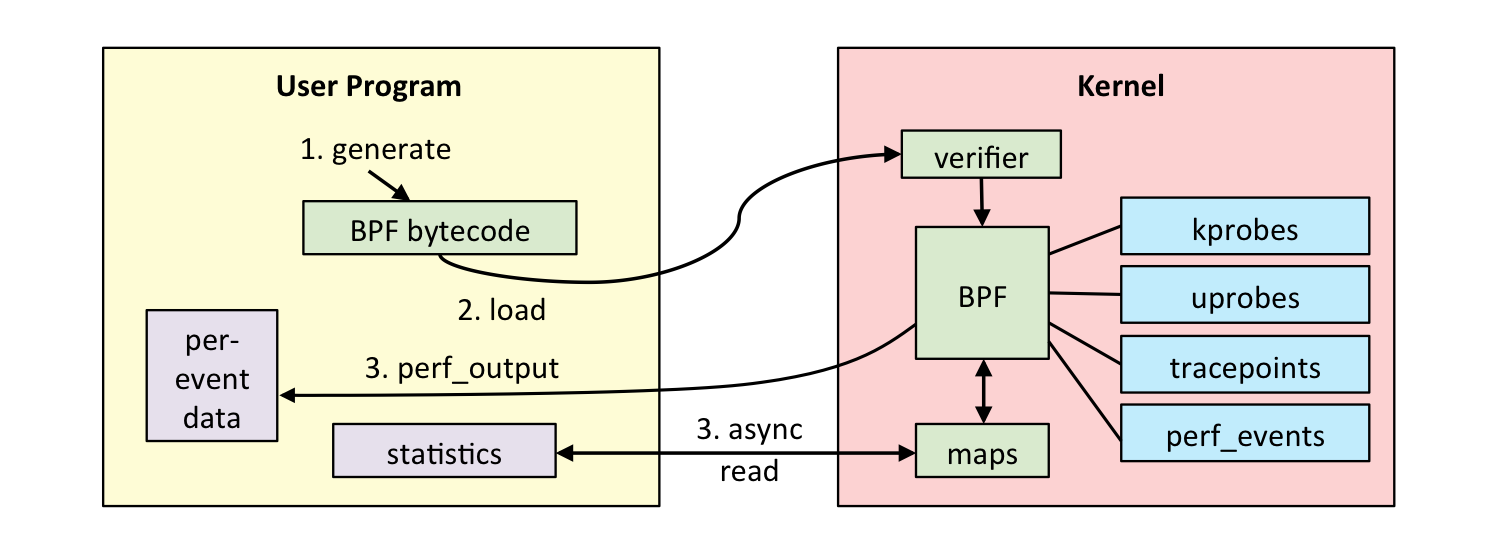
\includegraphics[scale=0.3]{images/linux_ebpf_internals}
  \caption{Detalle de como funciona un programa \emph{eBPF} y su relación con el kernel. \emph{Autor: Brendan Gregg}}
  \label{fig:ebpf-internals}
\end{figure}

el proyecto \emph{bcc} incluye pequeñas utilidades que sirven para monitorizar algunas partes del sistema, en la figura \ref{fig:bcc-tracing-tools} puede observarse un diagrama que incluye algunas de ellas
con referencia al sistema que monitorizan.

\begin{figure}[h]
  \centering
    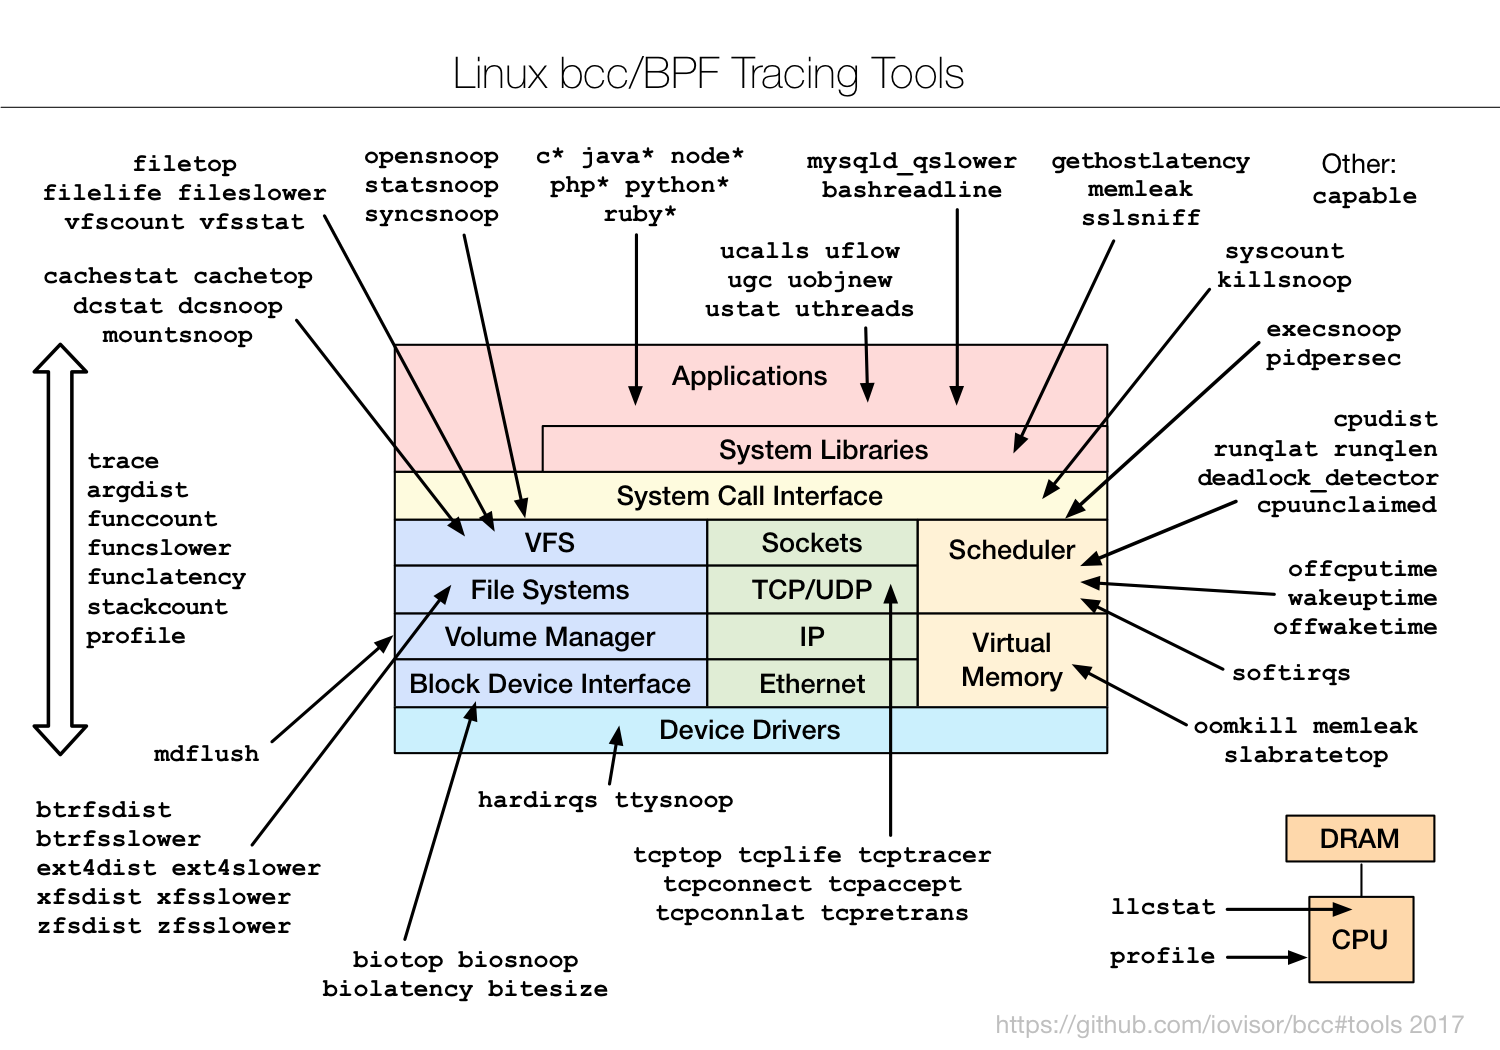
\includegraphics[scale=0.65]{images/bcc_tracing_tools}
  \caption{Relación de utilidades \emph{bcc} y subsistemas monitorizados. \emph{Autor: Brendan Gregg \& iovisor project}}
  \label{fig:bcc-tracing-tools}
\end{figure}

\begin{figure}[h]
  \centering
    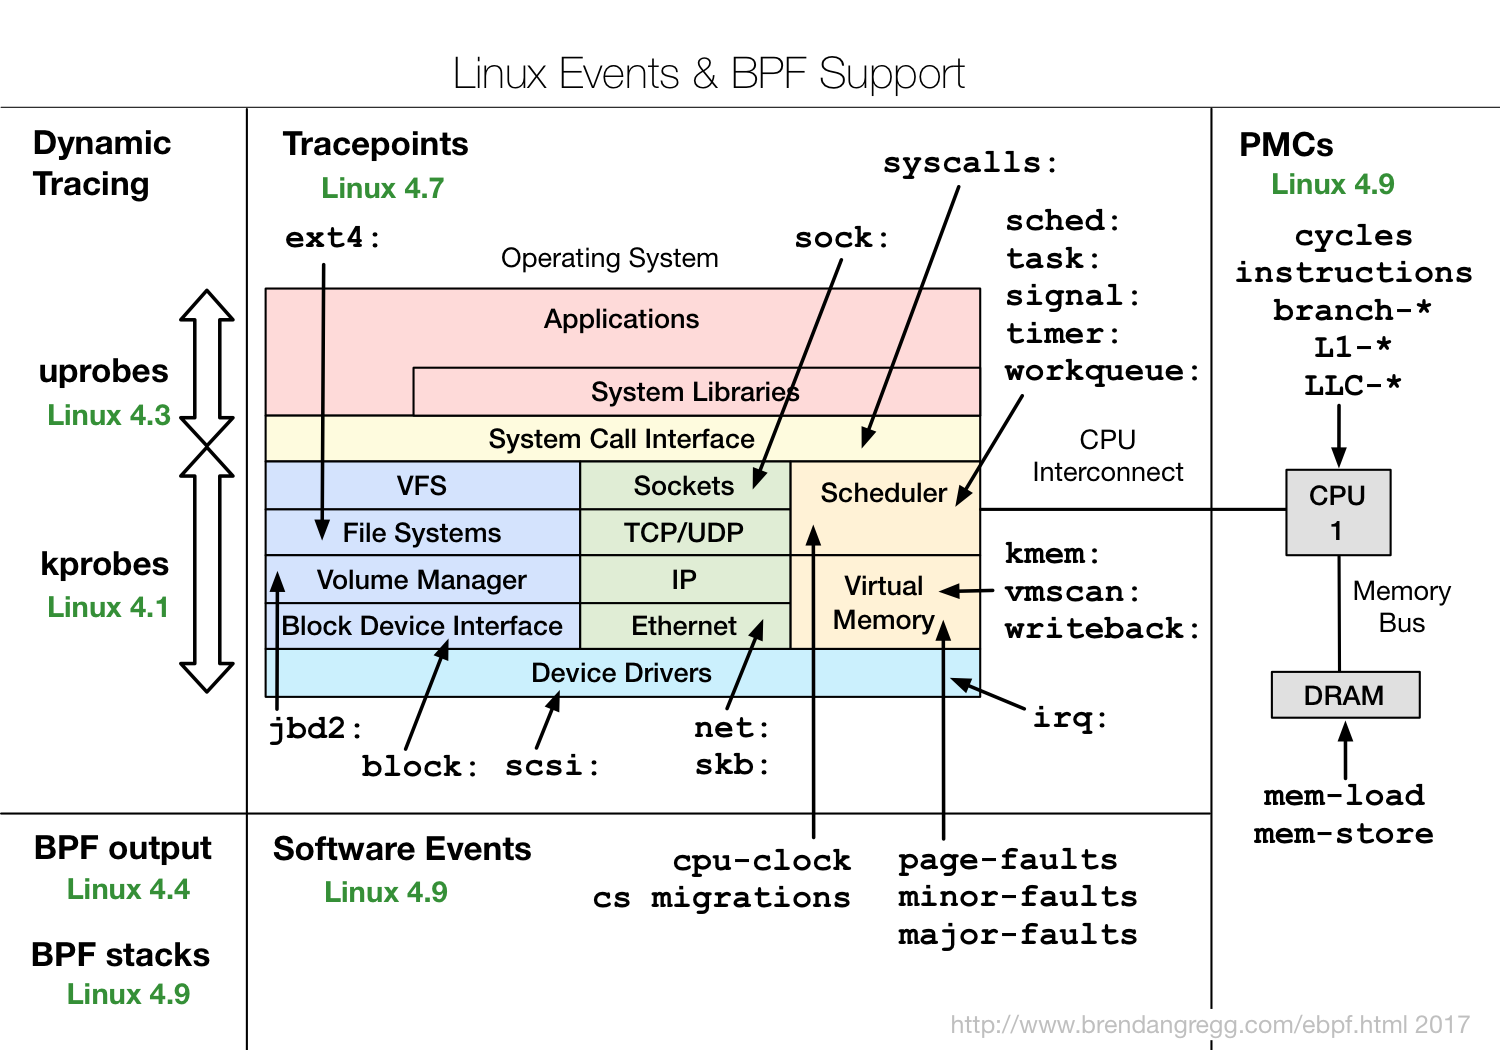
\includegraphics[scale=0.65]{images/linux_ebpf_support}
  \caption{Relación de versiones del kernel donde se dan soporte a susbsistemas en \emph{eBPF}. \emph{Autor: Brendan Gregg \& iovisor project}}
  \label{fig:linux_ebpf_support}
\end{figure}

\begin{table}[h]
\centering
\begin{tabular}[!h]{|l|}
\hline
Linux 4.12 Released 2 July, 2017 \\
\hline
Linux 4.11 Released 30 April, 2017 \\
\hline
Linux 4.10 Released 19 February, 2017 \\
\hline
Linux 4.9 Released 11 December, 2016 \\
\hline
Linux 4.8 Released 2 October, 2016 \\
\hline
Linux 4.7 Released 24 July, 2016 \\
\hline
Linux 4.6 Released 15 May, 2016 \\
\hline
Linux 4.5 Released 13 March, 2016 \\
\hline
Linux 4.4 Released 10 January, 2016 \\
\hline
Linux 4.3 Released 1 November, 2015 \\
\hline
Linux 4.2 Released 30 August, 2015 \\
\hline
Linux 4.1 Released 21 June, 2015 \\
\hline
Linux 4.0 Released 12 April, 2015 \\
\hline
\end{tabular}
\caption{\label{tab:linux-release-date}Fecha de publicación de versiones de Linux \emph{4.X}}
\end{table}

Sin embargo el soporte a subsistemas ha sido introducido de manera paulatina, desde la introducción de eBPF, como referencia véase el cuadro \ref{tab:linux-release-date} dónde se incluye la fecha de publicación de algunas versiones de la rama
\emph{4.x} y la figura \ref{fig:linux_ebpf_support} donde se aprecia en que versión del kernel se incluye.

\clearpage


Si se utiliza \emph{eBPF} hay importantes ventajas e incovenientes con respecto a \emph{auditd} y otras opciones:
\begin{enumerate}
    \item[Eficiencia] el procesado de eventos y filtrado se hace dentro del kernel, en un entorno aislado, lo que es mucho más
    rapido y menos costoso que copiar el evento a espacio de usuario y filtrarlo alli.
    \item[Prometedor] aunque \emph{eBPF} es de incorporación reciente utiliza tecnología existente en el kernel desde hace más de 20 años.
    \item[Falta de soporte] no hay que perder la vista de que queremos instrumentar una \emph{honeypot} y aunque es viable escribir aplicaciones \emph{eBPF} capaces de instrumentar, no hay demasiada documentación al respecto
    y quizá ese objetivo sea merecedor de un proyecto por sí sólo.
    \item[Soporte reciente] si queremos utilizar todas las capacidades de \emph{eBPF} necesitaremos al menos un kernel \emph{4.10} que no está disponible aún en todas las distribuciones, que suelen instalar
    versiones \emph{LTS} (4.4 actualmente) y que por lo tanto no estará disponible en la mayoría de proveedores de servidores como \emph{AWS, Digital Ocean \ldots}. Aunque no es imposible instalar nuevas versiones del kernel,
    supone un esfuerzo extra y un coste para el proyecto.
\end{enumerate}

Por éstas razones se descarta el uso de \emph{eBPF} que aunque prometedor aún no es suficientemente estable para acometer éste proyecto.
\clearpage

\subsection{Obteniendo información del kernel: crear un módulo}

Dado que por las razones expuestas extraer información vía interfaces externas no parecía factible, hay que explorar otras opciones.
el kernel de \emph{Linux} es modular, y por tanto se puede inyectar un módulo de codigo que extienda las capacidades del kernel, es la manera
en que habitualmente se cargan nuevos controladores, por ejemplo.

Ya que extraer información a través de interfaces conocidas no es factible, queda la opción de crearnos la nuestra propia. 
Desarrollar un módulo del kernel para generar eventos y procesarlos no es una tarea sencilla, el módulo debe ser eficiente para procesar el volumen
de eventos y correcto para no provocar un fallo en el kernel que deje inutilizado el sistema.

El esfuerzo y tiempo a dedicar necesario para crear un módulo de kernel con cierta calidad y caracteristicas necesitaria un tiempo de desarrollo grande, quizás de la talla
de éste mismo proyecto. Por ello, antes de comenzar esa tarea cabe buscar si hay opciones disponibles que nos eviten ese trabajo extra.

\emph{sysdig} (\cite{sysdig-project}) es un proyecto de \emph{Draios} que consta de una \emph{CLI (Command Line Interface)} que utiliza eventos de un modulo del kernel
licenciado con GPLv2, lo que supone un encaje perfecto para las necesidades del proyecto.

Ventajas e inconvenientes de éste enfoque:

\begin{enumerate}
    \item[Coste] Sysdig obtiene los eventos en espacio del kernel pero los copia a espacio de usuario para ser
    filtrados y procesados. Si el filtro que escogemos es suficientemente amplio se necesitará una importante cantidad de recursos de CPU y memoria para el filtrado y procesado de eventos.
    \item[Flexibilidad] \emph{sysdig} como cliente del modulo del kernel, proporciona una enorme flexibilidad a la hora de definir filtros y varios formatos de salida (JSON, formato variable \emph{a la printf},\ldots).
    \item[Almacenaje] \emph{sysdig} guarda a disco las trazas en fichero en un formato binario propio que es posible leer y filtrar con posterioridad. Proporciona además opciones para el rotado automático por tamaño y/o fecha,
    lo que permite el almacenaje y gestion de ficheros de trazas directamente desde sysdig y la capacidad de reprocesar eventos si los filtros originales son generalistas. 
\end{enumerate}

Las ventajas superan los incovenientes en éste caso, ya que aunque el consumo de CPU sea más elevado, poder gestionar las trazas directamente, reprocesar ficheros de captura y las opciones flexibles de filtrado y postprocesado hacen de ésta opción la opción finalmente escogida.

\subsection{Notificación de alertas en base a eventos capturados en las trazas}

Una vez que hemos establecido como obtener los eventos, necesitamos que en ciertas condiciones algun componente, ya
sea el método de instrumentación o un sistema externo nos notifique cuando se vulnera nuestra \emph{honeypot} o hay un
cambio relevante dentro de ella.

Necesitamos esa notificación para conocer cuando se produce un incidente y sobre todo para ser capaz de limpiar el entorno tras una
cierta ventana de tiempo de exposición, nuestro objetivo es el de aprender de nuestros atacantes no de convertirnos en una plataforma de soporte
para ellos.

Desgraciadamente, al comienzo de éste proyecto (Marzo de 2016) no existía ningún tipo de aplicación que realizase ésta tarea.
Por ello, extender \emph{sysdig} para realizar ésta tarea parece lo más apropiado, la manera de extension puede ser a través de un
script en Lua que sea ejecutado dentro de \emph{sysdig} o procesando la salida en una aplicación externa.

\emph{Lua} es un lenguaje pequeño, versatil y potente y posiblemente capaz de realizar ésta tarea, pero la poca familiaridad del autor con este lenguaje decanta
la balanza a favor de desarrollar una aplicación externa que recibiendo los eventos procesados por \emph{sysdig} genere las notificaciones.

Afortunada (o desgraciadamente por el tiempo \emph{invertido}) antes de que el desarrollo de dicha aplicación terminase, \emph{Draios} lanza \emph{Falco} (\cite{falco-project}) en Mayo de 2016, un proyecto cuyo objetivo
es el analizar el comportamiento anomalo de containers en base a filtros de \emph{sysdig} y generar notificaciones sobre ello.

El encaje con los propositos del proyecto es perfecto, y por ello se descarta el desarrollo propio tras una prueba inicial.

\subsection{Modelo de riesgo de la sonda y del servicio expuesto.}

El objetivo de una  \emph{honeypot} es el de engañar a atacantes para que realicen un ataque como lo harian en un entorno real. Aunque este ataque se produce en un entorno en el que esperamos un ataque
tendremos que definir el riesgo que asumimos al exponerse y que medidas o politicas se aplicarán para éstos riesgos. En la figura \ref{fig:riesgo_sonda} se describen los posibles riesgos, realizando un diagrama de riesgos siguiendo la metodologia expuesta en \cite{Shostack:2014:TMD:2829295}.

\begin{figure}[!h]
  \centering
    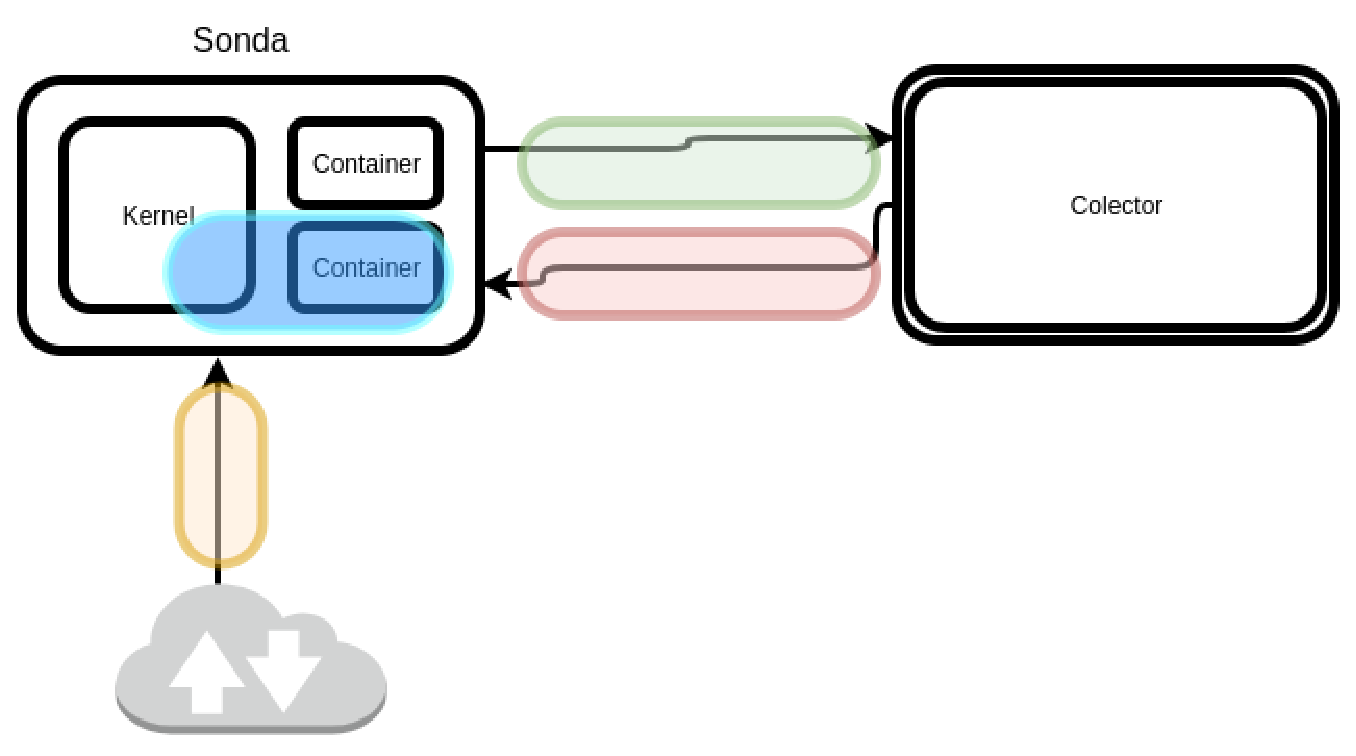
\includegraphics[scale=0.4]{images/threat_model_probe}
  \caption{Modelo de riesgo de la sonda}
  \label{fig:riesgo_sonda}
\end{figure}

Listado de riesgos analizados sobre la figura \ref{fig:riesgo_sonda}:
\begin{enumerate}
    \item[\emph{Naranja 1}] Elevación de privilegios atacando a un servicio expuesto que no pertenece a la \emph{honeypot}. Un atacante puede explotar un servicio de soporte como un servidor SSH de administración o un servicio interno expuesto por mala configuración.
    \item[\emph{Naranja 2}] Riesgo de que la \emph{honeypot} sea reconocible o listada, la \emph{honeypot} es conocida por alguna caracteristica (\emph{IP del servidor, versión del servicio,\ldots}) marcandola como \emph{honeypot} permitiendo a los atacantes simplemente ignorarla.
    \item[\emph{Azul}] El atacante escapa desde el \emph{container}, elevación de privilegios que rompe el aislamiento del kernel y el atacante gana acceso a otros containers o al servidor.
    \item[\emph{Verde}] \emph{Spoofing} de la información enviada al colector, una vez el atacante gana acceso al servidor puede enviarnos al colector información falseada.
    \item[\emph{Rojo}] Elevación de privilegios de un atacante que ya ha conseguido acceso al colector. El colector y la sonda mantendran una conexión, si alguien ataca al colector y gana privilegios puede atacar a las sondas. Pese a que es un riesgo, si el colector ha sido vulnerado, que nos ataquen las sondas no es tan grave.
\end{enumerate}

Listado de mitigaciones para los riesgos analizados:
\begin{enumerate}
    \item[\emph{Naranja 1}] Reducir la superficie de ataque, eliminar servicios expuestos que no pertenezcan a la \emph{honeypot} o limitar el acceso a ciertas direcciones ip conocidas.
    \item[\emph{Naranja 2}] Para mitigar este riesgo, las versiones de las aplicaciones expuestas deben estar ocultas o ser indistinguibles. la mejor alternativa para mitigar éste riesgo es reciclar las sondas, y crear sondas nuevas con suficiente frecuencia. Si el sistema de provisionamiento y configuración de sondas es automatico, se pueden crear nuevas sondas con frecuencia diaria u horaria.
    \item[\emph{Azul}] Debemos aceptar el riesgo, que el container siempre tendra acceso al kernel que se comparte con otros containers y el servidor, como mitigación podemos restringir los privilegios del container para que solo pueda utilizar algunas syscalls, pero en cualquier caso el riesgo de compromiso de un servidor a traves de un container siempre estara presente. 
    \item[\emph{Verde}] La comunicacion entre sonda y colector se realizara a traves de un canal cifrado con clave asimetrica. En el lado del colector se pueden realizar validaciones de entrada antes de guardar en base de datos o actuar sobre los eventos recibidos.
    \item[\emph{Rojo}] De todos los riesgos listados, este es el menos grave, si el colector ha sido atacado y vulnerado tendremos problemas mayores que nuestra sonda sea atacada.
\end{enumerate}

\subsection{Securizacion de la sonda}

% medidas en el host,
% mover ssh de gestion a otro puerto.
% actualizacion de paquetes de seguridad.
% reducir al minimo software.
% limitacion del ancho de banda de los containers
% apparmor y seccomp en containers.

% 18/08/2017

% % Sonda,
%  * como instrumentar los containers, via interfaces conocidas.
%  * LXC vs Docker vs rkt.
%  * Auditd, netlink, KLM.
%  * Notificaciones de trazas.
%  * Modelo de seguridad de la sonda y del servicio expuesto.
%  * limitacion del ancho de banda de la red para limitar usando TC.
%  * Securizacion de la sonda.

% 19/08/2017

% % Collector,
%  * registro de las sondas
%  * coleccion de alertas de Falco.
%  * coleccion de trazas del sistema.
%  * Procesamiento de trazas del sistema 
%  * Almacenamiento de informacion

% 20/08/2017


% API
%  * exposicion de la información.
%  * Arquitectura de la API / versionado
%  * REST vs GRAPHQL

\section{Resultados finales}

% 25/08/2017

% Arquitectura
%  * Descripcion de la arquitectura.
%  * Registro de las sondas.
%  * Notificacion de nuevas trazas.
% Despliegue
%  * Mantenimiento de la arquitectura usando Ansible.

\section{Planificación}

% 26/08/2017

% Commit inicial 15/2/2016
% Prototipo 21/5/2016
% Construccion de la sonda 21/5/2016 - 20/5/2017
% Construccion del colector 20/5/2016 - 21/7/2016
% Construccion de la API 21/7/2016 - 22/7/2016

\subsection{Metodologia utilizada: modelo iterativo}
% 27/08/2017

%%% Local Variables: 
%%% mode: latex
%%% TeX-master: "main"
%%% End: